
\documentclass{article}
\usepackage[utf8]{inputenc}
\usepackage{graphicx}
\usepackage{listings}
\usepackage{xcolor}
\usepackage{float}  % Add float package to control figure placement
\usepackage{amsmath}

\title{08b Stepper Motor Introduction}
\author{Nicholas Bruzzese}
\date{\today}

\definecolor{dkgreen}{rgb}{0,0.6,0}
\definecolor{gray}{rgb}{0.5,0.5,0.5}
\definecolor{mauve}{rgb}{0.58,0,0.82}

\lstset{frame=tb,
	language=Python,
	aboveskip=3mm,
	belowskip=3mm,
	showstringspaces=false,
	columns=flexible,
	basicstyle={\small\ttfamily},
	numbers=none,
	numberstyle=\tiny\color{gray},
	keywordstyle=\color{blue},
	commentstyle=\color{dkgreen},
	stringstyle=\color{mauve},
	breaklines=true,
	breakatwhitespace=true,
	tabsize=3
}

\begin{document}
	
	\maketitle
	
	\section*{What is a Stepper Motor?}
	A stepper motor is a type of DC motor that moves in discrete steps. Unlike regular motors that spin continuously when powered, stepper motors are designed to:
	\begin{itemize}
		\item Rotate in precise increments.
		\item Maintain their position when not moving.
		\item Be controlled for speed, direction, and step count.
	\end{itemize}
	
	\subsection*{Key Features}
	\begin{itemize}
		\item \textbf{Steps per Revolution}: Defines how many steps the motor takes to complete one full rotation.
		\item \textbf{Direction Control}: Easily reversible rotation.
		\item \textbf{Precision}: Ideal for applications requiring accurate positioning, like 3D printers or camera sliders.
	\end{itemize}
	
	\section*{Hardware Requirements}
	\begin{itemize}
		\item Raspberry Pi (any model with GPIO pins).
		\item 28BYJ-48 stepper motor with ULN2003 driver board.
		\item Jumper wires for connections.
	\end{itemize}
	
	\section*{Wiring Diagram}
	\begin{figure}[H]
		\centering
		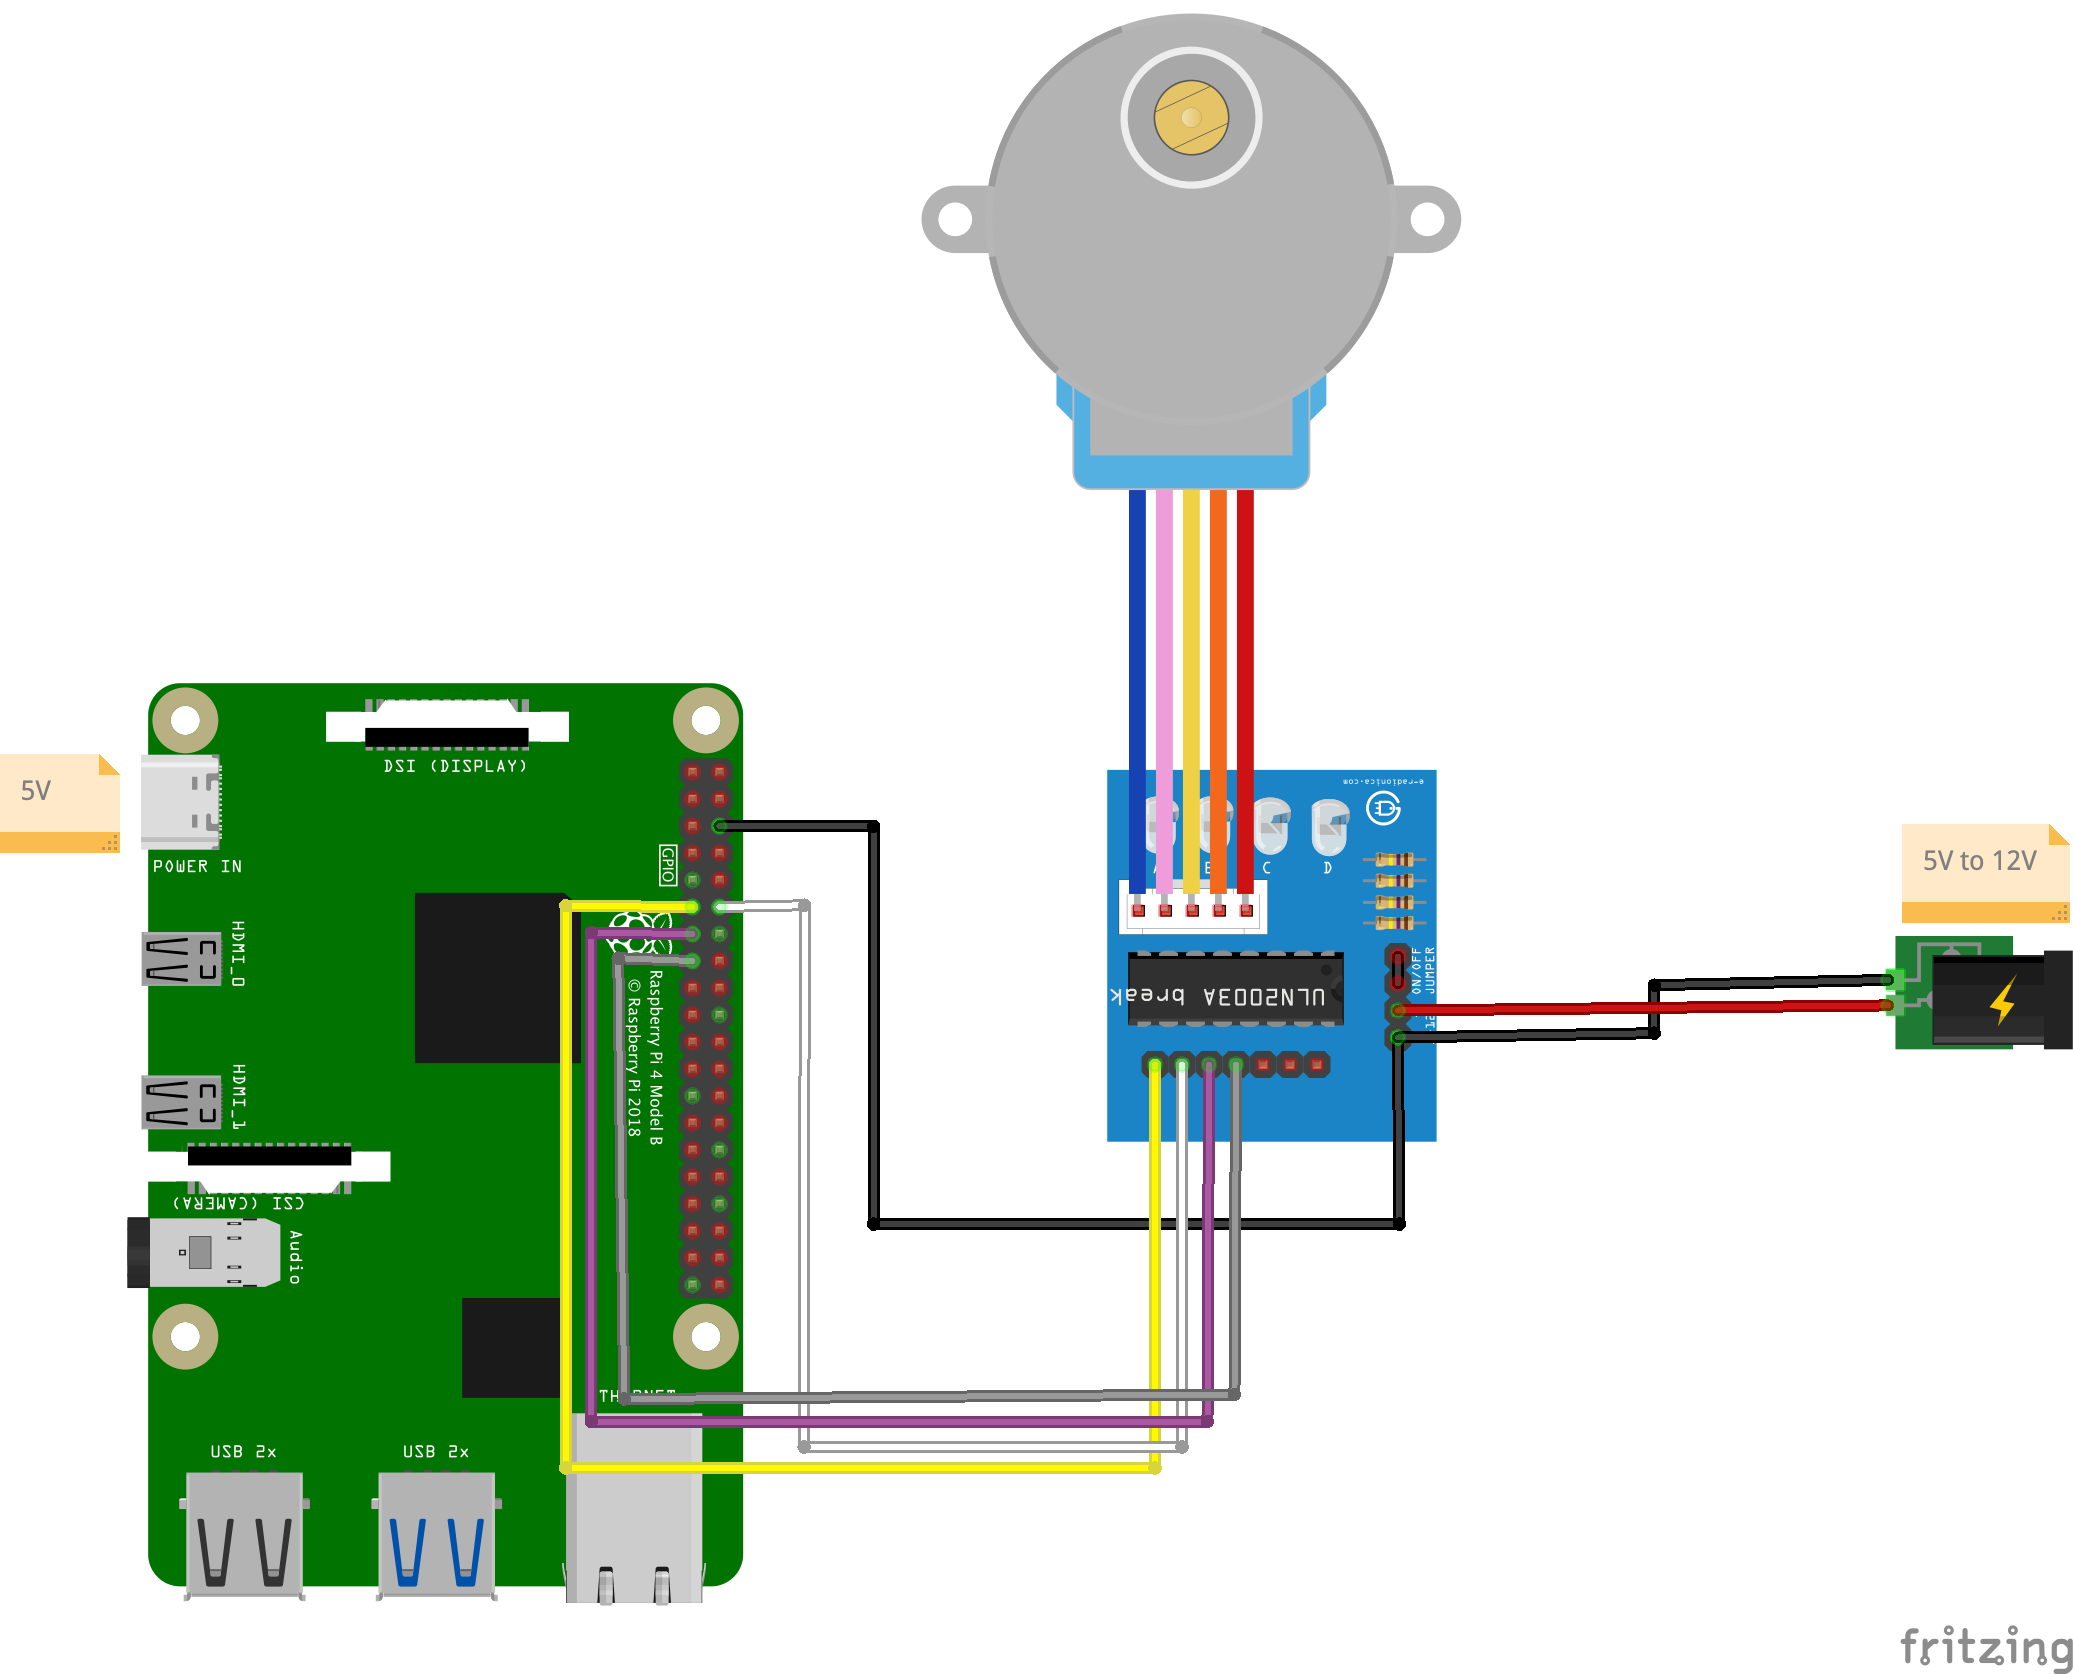
\includegraphics[width=1.2\textwidth]{08b-stepper-motor-diagram.png} % Adjust width to 80% of text width
		\caption{Wiring Diagram}
	\end{figure}
	
	\section*{Stepper Motor Setup with Raspberry Pi}
	\subsection*{Connections}
	\begin{itemize}
		\item Connect the \texttt{IN1, IN2, IN3, IN4} pins of the ULN2003 driver board to GPIO pins \texttt{17, 18, 27, and 22} of the Raspberry Pi.
		\item Connect \texttt{VCC} on the driver board to the 5V pin of the Raspberry Pi.
		\item Connect \texttt{GND} on the driver board to a GND pin of the Raspberry Pi.
	\end{itemize}
	
	\section*{Python Code Explanation}
	
	The following Python code controls the stepper motor by sending precise signals to its pins. Let’s break it down:
	
	\subsection*{Setup}
	Define GPIO pins to control the motor and initialize the GPIO settings.
	
	\begin{lstlisting}
		import RPi.GPIO as GPIO
		import time
		
		# Pin definitions
		in1 = 17
		in2 = 18
		in3 = 27
		in4 = 22
		
		# GPIO setup
		GPIO.setmode(GPIO.BCM)
		GPIO.setup(in1, GPIO.OUT)
		GPIO.setup(in2, GPIO.OUT)
		GPIO.setup(in3, GPIO.OUT)
		GPIO.setup(in4, GPIO.OUT)
		GPIO.output(in1, GPIO.LOW)
		GPIO.output(in2, GPIO.LOW)
		GPIO.output(in3, GPIO.LOW)
		GPIO.output(in4, GPIO.LOW)
	\end{lstlisting}
	
	\subsection*{Stepper Motor Sequence}
	The stepper motor rotates when its coils are energized in a specific sequence.
	
	\begin{lstlisting}
		step_sequence = [[1,0,0,1],
		[1,0,0,0],
		[1,1,0,0],
		[0,1,0,0],
		[0,1,1,0],
		[0,0,1,0],
		[0,0,1,1],
		[0,0,0,1]]
	\end{lstlisting}
	
	\subsection*{Motor Rotation Logic}
	The motor rotates based on:
	\begin{itemize}
		\item \textbf{Step Count}: Total steps for one full rotation (e.g., 4096 for the 28BYJ-48 motor).
		\item \textbf{Direction}: Clockwise (CW) or Counterclockwise (CCW).
		\item \textbf{Sleep Time}: Time delay between steps controls motor speed.
	\end{itemize}
	
	\begin{lstlisting}
		step_sleep = 0.002  # Delay between steps
		step_count = 4096   # Total steps for one full rotation
		direction = False   # False for CCW, True for CW
		
		motor_pins = [in1, in2, in3, in4]
		motor_step_counter = 0
	\end{lstlisting}
	
	\subsection*{Main Loop}
	The loop iterates through the steps, updating the motor's state based on the step sequence.
	
	\begin{lstlisting}
		try:
		for i in range(step_count):
		for pin in range(0, len(motor_pins)):
		GPIO.output(motor_pins[pin], step_sequence[motor_step_counter][pin])
		motor_step_counter = (motor_step_counter + 1) % 8 if not direction else (motor_step_counter - 1) % 8
		time.sleep(step_sleep)
		except KeyboardInterrupt:
		pass
		finally:
		GPIO.cleanup()
	\end{lstlisting}
	
	\section*{Running the Code}
	Save the code as \texttt{stepper\_motor.py} and run it using the command:
	\begin{lstlisting}
		python3 stepper_motor.py
	\end{lstlisting}
	
	\subsection*{Expected Behavior}
	\begin{itemize}
		\item The motor will rotate 360° in 4096 steps.
		\item To reverse the direction, set \texttt{direction = True} in the code.
	\end{itemize}
	
	\section*{Experiment Ideas}
	\begin{itemize}
		\item \textbf{Speed Control}: Change \texttt{step\_sleep} to see how it affects speed.
		\item \textbf{Partial Rotations}: Adjust \texttt{step\_count} for specific angles (e.g., 90° = 1024 steps).
		\item \textbf{Interactive Control}: Use user input to set the direction or steps dynamically.
	\end{itemize}
	
\end{document}
